% this is not genereated from Markdown so the edits can be here
\section{Register based Virtual Machine}
\crexx{} uses a register based virtual machine.
A \index{register-based virtual machine} uses registers, which are memory locations, to store and manipulate data. In a register-based virtual machine, the instructions explicitly reference the registers by number, and the values are loaded into and out of the registers as needed. This approach can provide faster performance because accessing registers is typically faster than accessing memory. In the \emph{rxvm} virtual machine, the compiler of the underlying C implementation assigns the hardware registers.

In contrast, a \index{stack-based virtual machine} uses a stack to store and manipulate data. In a stack-based virtual machine, the operands are pushed onto the stack, and the operators pop them off the stack, perform the operation, and push the result back onto the stack. The stack-based approach is simpler than the register-based approach because there are no explicit references to registers in the instructions, and the operands are automatically managed by the stack. However, the stack-based approach can be slower than the register-based approach because accessing memory is typically slower than accessing registers.

Some other differences between a register-based virtual machine and a stack-based virtual machine include:
\begin{itemize}
\item Register-based virtual machines typically use more memory for the registers than stack-based virtual machines use for the stack.
\item Register-based virtual machines may require more complex instruction encoding and decoding logic than stack-based virtual machines, which can impact the size and complexity of the virtual machine implementation.
\item Stack-based virtual machines can be easier to implement and optimize for certain types of operations, such as function calls and loops, where the data can be easily pushed onto and popped off the stack.
\item Register-based virtual machines can provide more flexibility in terms of register allocation and optimization, which can be particularly important for high-performance applications.
\end{itemize}

The execution environment of a \crexx{} program is a
threaded\footnote{an alternative, non-threaded executable is available
  under the \emph{\index{rxbvm}} name} virtual
machine that is designed for optimal performance. This virtual
machine, implemented in the \emph{rxvm} executable, executes
machine instructions produced by the \emph{rxc} \crexx{}
compiler, or written by hand, assembled into an .rxbin binary file by
the \emph{rxas} assembler.

\section{REXX VM Specification}

\emph{Page Status: This page is work in progress, incomplete, inconsistent and full of errors ... read with care!}

\subsection{Acknowledgement}

Much of this work is based on the excellent \textquotedbl{}Language Implementation Patterns\textquotedbl{}
by Terence Parr.

https://pragprog.com/titles/tpdsl/language-implementation-patterns/

\subsection{REXX VM Components - Summary}

The REXX interpreter simulates a computer with the following components:

\begin{itemize}
\item Code memory: This 64 or 32-bit unsigned integer array holds a program's \textquotedbl{}bytecode\textquotedbl{} instructions
(bytecodes plus operands). Addresses are integers.

\item ip register: The instruction pointer is a special-purpose ``register'' that
points into code memory at the next instruction to execute.

\item CPU: To execute instructions, the interpreter has a simulated CPU that
conceptually amounts to a loop around a giant ``switch on bytecode'' statement.
This is called the instruction dispatcher. We will use a Threaded VM instead.

\item Constant pool: Anything that we can't store as an integer operand
goes into the constant pool. This includes strings, arbitrary precision numbers,
and function symbols. Instructions like \texttt{say {[}STRING{]}} and use an index into
the constant pool instead of the actual operand.

\item Function call stack: The interpreter has a stack to hold function call return
addresses as well as parameters and local variables.

\item fp register: A special-purpose register called the frame pointer that points
to the top of the function call stack. StackFrame represents the information
we need to invoke functions.

\item An infinite and regular register set per function call. Functions can access
any element in the register array, whereas a stack can only access elements
at the end. Registers hold integer, float, string and object values, plus flags
that can be used to dynamically store which value formats are valid.

\end{itemize}

The following capabilities will be implemented in REXX Level B - REXX called by the virtual machine

\begin{itemize}
\item Variable Pool: Holds slots for variables, each function/procedure has its own
pool, and a function/procedure can \textquotedbl{}link\textquotedbl{} to variables from the parents pool (to
support dynamic expose scenarios).
The memory slots can point at Integer, Float, String, and struct instances.
Variables are accessed via a linked register. This linking can be done statically
or dynamically via a variable search capability

\item Runtime libraries that care used as \textquotedbl{}exits\textquotedbl{}; for example, REXX code to format error messages.

\end{itemize}

\subsection{REXX Machine Architecture}

cREXX will target a bytecode interpreter tuned for the specific needs of
the REXX language. This has two advantages

\begin{itemize}
\item Provides platform independence and portability

\item Provides a much simpler target for the cREXX compile compared to real CPU\textquotesingle{}s
instruction sets (which after all have to be implemented in hardware)

\end{itemize}

A bytecode interpreter is like a real processor. The biggest difference is
that bytecode instruction sets are much simpler. Also, for example, we can
assume there are an infinite number of registers.

The cREXX VM is a register based bytecode interpreter that uses Threading
and Super-Instructions, meaning:

\subsubsection{Register Based}

A Register Based VM instructions use registers. The cREXX VM gives each
stack frame an ``infinite'' set of registers.

\subsubsection{Threading}

Threading means that the \textquotedbl{}bytecode\textquotedbl{} loader converts instruction opcodes to
the address of the subroutine that emulates the instruction. This reduces
an indirection to each instruction (i.e. instead of
\texttt{switch(opcode) \{case ...\})} we can do \texttt{goto opcode\_address}).

In addition, the code to dispatch to the next instruction is repeated at the
end of each instruction subroutine rather than having a single dispatcher.
This allows the real CPU\textquotesingle{}s pipelining logic to work better.

The following two examples demonstrate the concept.

\paragraph{Traditional Interpreter}

\begin{verbatim}
char code[] = {
  ICONST_1, ICONST_2,
  IADD, ...
}
char *pc = code;

/* dispatch loop */
while(true) {
  switch(*pc++) {
    case ICONST_1: *++sp = 1; break;
    case ICONST_2: *++sp = 2; break;
    case IADD:
      sp[-1] += *sp; --sp; break;
   ...
  }
}
\end{verbatim}

\paragraph{Equivalent Threaded Interpreter}

\begin{verbatim}
void *code[] = {
  &&ICONST_1, &&ICONST_2,
  &&IADD, ...
}
void **pc = code;

/* implementations */
goto **(pc);

ICONST_1: pc++; *++sp = 1; goto **(pc);
ICONST_2: pc++; *++sp = 2; goto **(pc);
IADD:
  pc++; sp[-1] += *sp; --sp; goto **(pc);
...
\end{verbatim}

Note how the next instruction pointer \texttt{pc} is calculated up front (\texttt{pc++}) before
the instruction logic. This is to allow the CPU pipeline to work; by the
time the \texttt{goto} is being decoded the value of \texttt{pc} \emph{should} have completed.

\subsubsection{Super Instructions}

In any interpreter the dispatch to the next instruction is an overhead. The
fewer instructions needed to execute logic then the less dispatching overhead.
Moreover a complex instruction\textquotesingle{}s native implementation code running linearly
maximises the effectiveness of the real CPU\textquotesingle{}s pipeline.

We therefore will have a large number of instructions to cater for common
sequences, for example a decrement (decr) instruction might often be followed by a
branch if not zero instruction (brnz), e.g. for a loop - a super-instruction combines
these two instructions to one (e.g. decrbrnz).

\subsubsection{Low-level Function Instructions}

The VM provides low-level functions as instruction, for example covering
aspects like variable manipulation (like substr()), IO functions,
Environment access, and virtual hardware like the timer. This ensures that:

\begin{itemize}
\item Platform independence / platform drivers / porting etc. is
achieved only by implementing these instructions for each platform.

\item Higher level functionality can all be implemented in REXX.

\end{itemize}

\subsubsection{Instruction coding}

There is a balance here - memory usage verses performance, made more complicated
because reducing memory usage also has performance benefits. Tests will be
needed across different CPUs types to validate our optimisations.

\paragraph{Compiled Mode}

REXX VM binary code can be generated for storage (i.e. compiled) to be loaded
and run later. In this case the code will have to be loaded and then threaded.

The threading process converts the op\_codes into addresses, branches to addresses
constant indexes to addresses - everything is converted into real addresses
of the machine running the REXX VM, so that when executed (for example) data is
accessed via its real address with no lookups/indexes needed. This needs to
be all done at load time as the exact real addresses will be different on each machine
and for each run (modern OS\textquotesingle{}s randomise load addresses).

We will investigate if there is value in compressing the saved REXX VM binary
to speed load times. Java uses ZIP for this and cREXX could do the same - and/or
we could pack the instruction coding.

In the short term we will save it as 32 or 64 bit instructions (see following).

This means that the threading process can simply
replace the opcode with the opcode address - the 32 or 64 bit memory address can
fit in the 32 or 64 bit int instruction code location, we overwrite the opcode
integer with the opcode function address.

\paragraph{Interpreter Mode}

When interpreting a REXX program the compiler will emit code that will be
executed there and then. In principle all the real addresses will be known and
this means that the compiler can generate threaded code from the get-go. This
way the loading / threading stage can be skipped.

Initial versions will only use the Compiler Mode while the Interpreter Mode is
checked for feasibility and to see if there is a noticeable performance gain. One
issue we may have is that the loader/threader may be needed anyway for other reasons
like late binding/linking of libraries.

\paragraph{Endianness}

Where the compiler and runtime are known to be on the same machine then the
Endianness and float format will be machine specific.

Where the REXX VM is to be saved then big-endianness / \textquotedbl{}network order\textquotedbl{} will be
used. And for floats we will use big-endianness double (IEEE 754 / binary64).

The loader / threader will need to convert as need be.

\paragraph{32 / 64 bit}

Although we are only expecting a few hundred opcodes (if that!!), we need to store
them in an integer of the same size as the machine address pointer size because
of the need to overwrite the op\_code with its implementation address.

For a 64bit OS we therefore need to store all opcodes and register numbers as 64-bit
integers.

\textbf{Note: If not for threading, there could have been many schemes to compress this,
for example a 64bit integer could have held a 16-bit opcode and 3 16-bit register
numbers as parameters - very efficient. Therefore we will confirm that the
threaded interpreter is still faster than a classic interpreter using this more
efficient scheme. Modern CPU\textquotesingle{}s may be much smarter at pipelining!}

The 64 bit machine code format is therefore

\begin{itemize}
\item A 64bit Opcode, followed by

\item Zero or more (depending on opcode) 64bit parameters. Each parameter (depending on
the opcode) can be one of:

\begin{itemize}
\item An integer constant

\item An double float constant

\item Index to an item in the constant pool (e.g. a String, High-precision Number
or Object Constant)

\item Register Number

\item An instruction Number (i.e. a virtual address for a jump)

\end{itemize}

\end{itemize}

For 32-bit machines we can use two options

\begin{enumerate}
\item Have an alternative but equivalent format using 32bit integers/floats/addresses.
This reduces the size of binaries but reduces compatibility between 64-bit and
32-bit machines. 2 versions of binaries may be needed, or the loader could convert
on load. An issue is that Float constants would need to be put in the Constant
pool.

\item Use the 64-bit format for 32 bit machines. This means that 50\% of the program
space will be wasted but will provide compatibility. Note that only
4,294,967,295 registers per stack frame will be supported!

\end{enumerate}

We will explore the different options here including looking at program size
and performance.

\subsection{Standards/Rules for VM Instruction Implementation}

The following are the rules that should be followed when implementing VM Instructions.

\subsubsection{Key Principles}

\begin{enumerate}
\item To maximise CPU performance with respect to speculative execution (including simple pipelining) branches should be avoided and if required (e.g. when dispatching to the next instruction) the target address should be calculated and assigned as early as possible.

\item The compiler (or human writing the assembler code) is responsible for producing valid assembler including ensuring that assembler registers are initiated and have the required type, and ensuring (for example) then bound checks have been done. Run time validation at the VM Instruction levels should be avoided except for

\end{enumerate}

\begin{itemize}
\item When in debug mode

\item When \textquotedbl{}safe\textquotedbl{} versions of instructions are used by the compiler - see later.

\end{itemize}

Badly formed REXX Assembler code will have undefined runtime behaviour.

Justification for this approach is that SPECTRE attacks mean that it is possible for a program to access all process memory in a VM despite any access checks implemented by the VM (see Google\textquotesingle{}s SPECTRE JavaScript demonstrator).

For information, a SPECTRE attack uses the non-functional performance improvement of a data read associated with a speculative execution of an invalid instruction that moved data into the L1 cache. My assessment (and that of security advice) is that designers should assume untrusted code can read across an entire process memory space (and across a CPU core too) and that countermeasures will have limited impact because of the fundamental need for the performance boost provided by speculative execution and caches (we are not giving those up!)

Therefore when deploying cREXX code in a secure manner each VM instance will need to be in its own process space - and that is the way we will need to protect against nefarious code. All the cleaver work done in the Java and .NET VMs to prove code is safe might very well be proved to be pointless :-(

\subsubsection{Rules}

\begin{enumerate}
\item Calculate the next instruction address as early as possible.

\item Do not use \textquotedbl{}if\textquotedbl{} statements and validation

\item Conversion errors should cause SIGNALS (\textquotedbl{}goto SIGNAL;\textquotedbl{})

\item When needed by the compiler we will define large instructions that combine several instructions into one - this avoid multiple instruction dispatches.

\item Use DEBUG Macros to store debug validation - these will be not included in production/release compiled code.

\end{enumerate}


\section{\crexx{} Virtual Machine instructions}

% \section{Machine Interface}
This section describes the processor-specific information for the
hypothetical rxvm processor. \index{RXVM processor} The instruction set can be seen as the ISA
(instruction set architecture) for an RXVM processor, of which the microcode is implemented in the C99 language.

% \subsection{Processor Architecture}
\index{processor architecture}
\index{instruction set}
Programs intended to execute directly on the processor use the
RXVM instruction set and the
instruction encoding and semantics of this architecture.

An application program can assume that all instructions defined by the
architecture and that are neither privileged nor optional, exist and work
as documented.

To be ABI (application binary interface) conforming, the processor must implement the instructions of
the architecture, perform the specified operations, and produce the
expected results.  The ABI neither places performance constraints on
systems nor specifies what instructions must be implemented in
hardware.  A software implementation of the architecture conforms to
the ABI; likewise, the architecture could be implemented in hardware,
e.g. an FPGA.

\subsection{The Register}
\index{register}
\begin{wrapfigure}{l}{0.4\textwidth}
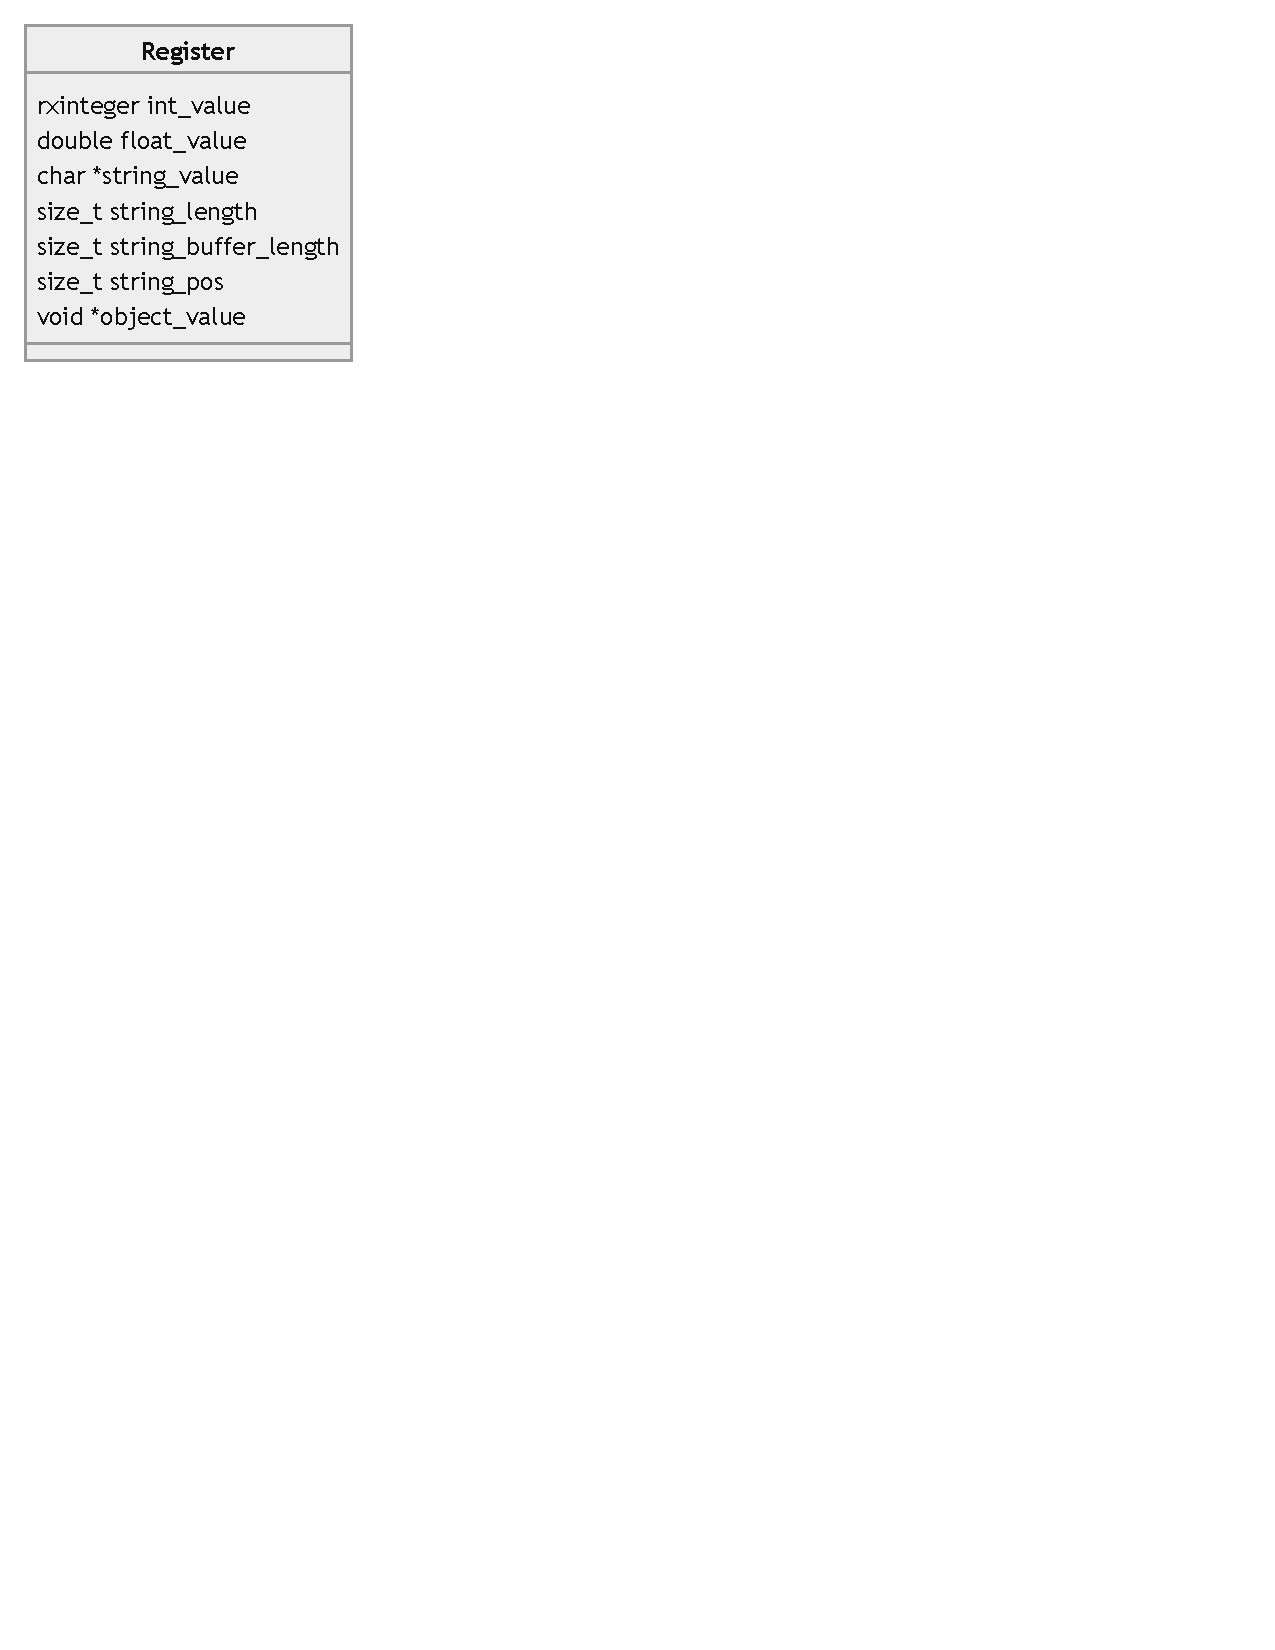
\includegraphics[scale=0.6]{charts/register.pdf}
\end{wrapfigure}


\crexx{} \code{rxvm} is a Register based virtual machine, as opposed to a Stack based
VM. The number of registers is only limited by memory and, for
practical purposes, can be considered unlimited. The address size of
the fields in a register is, for the virtual machine implementations,
implied by the address size that the host OS can handle. For hardware
the size is undefined and can follow the hardware address generation
capacity.


\begin{lstlisting}[label=crexxregister,caption={The
\crexx{} Register implementation in C}]
struct value {
    /* bit field to store value status - these are explicitly set */
    value_type status;

    /* Value */
    rxinteger int_value;
    double float_value;
    void *decimal_value; /* TODO */
    char *string_value;
    size_t string_length;
    size_t string_buffer_length;
    size_t string_pos;
#ifndef NUTF8
    size_t string_chars;
    size_t string_char_pos;
#endif
    void *object_value;
\end{lstlisting}

\subsubsection{Conversions of register values}
\index{conversions, data type in assembler}
\index{say instruction, rxas}
\index{int_value, register}
The status field determines for instructions that expect a data type,
which field is the field to act upon. Conversions are possible but
never implicit. So for example, when the register contains an int
value in field \code{int_value}, but it needs to be printed with the rxas
\keyword{say} instruction, the
\keyword{0\index{itos}} instruction takes care of the conversion and the population of the
memory area the \code{*string_value} points to. 

\begin{lstlisting}[label=crexxregister,caption={Values of
the Status field}]
typedef union {
    struct {
        unsigned int type_object : 1;
        unsigned int type_string : 1;
        unsigned int type_decimal : 1;
        unsigned int type_float : 1;
        unsigned int type_int : 1;
    };
    unsigned int all_type_flags;
} value_type;
\end{lstlisting}

